\section{Durchführung}
\label{sec:Durchführung}
Zur Durchführung des Experimentes wird der in \autoref{fig:Aufbau} gezeigte Versuchsaufbau verwendet. Licht aus einer Rubidium-Lampe wird fokussiert und über einen 
$\text{D}1$-Filter, sowie einen linear Polarisator und ein $\lambda/4$-Plättchen durch eine geheizte Rubidium-Kammer gelenkt.
Der Polarisator und das $\lambda/4$-Plättchen sind so angeordnet, dass nur rechtszirkular polarisiertes Licht durch die Kammer geleitet wird.
Am Ende des Aufbaus befindet sich eine weitere Linse und ein Photoelement mit dem die Lichtintensität (Transmission) gemessen werden kann.
Um die Rubidiumzelle befinden sich drei Helmholtzspulenpaare: Die Vertikalfeldspule, die Horizontalfeldspule und die Modulationsspule (Sweep-Spule),
welche parallel zur Horizontalfeldspule liegt.
Des Weiteren können ein Frequenzgenerator zur Erzeugung des RF-Feldes und ein Oszilloskop zur Messung angeschlossen werden.
\begin{figure}
    \centering
    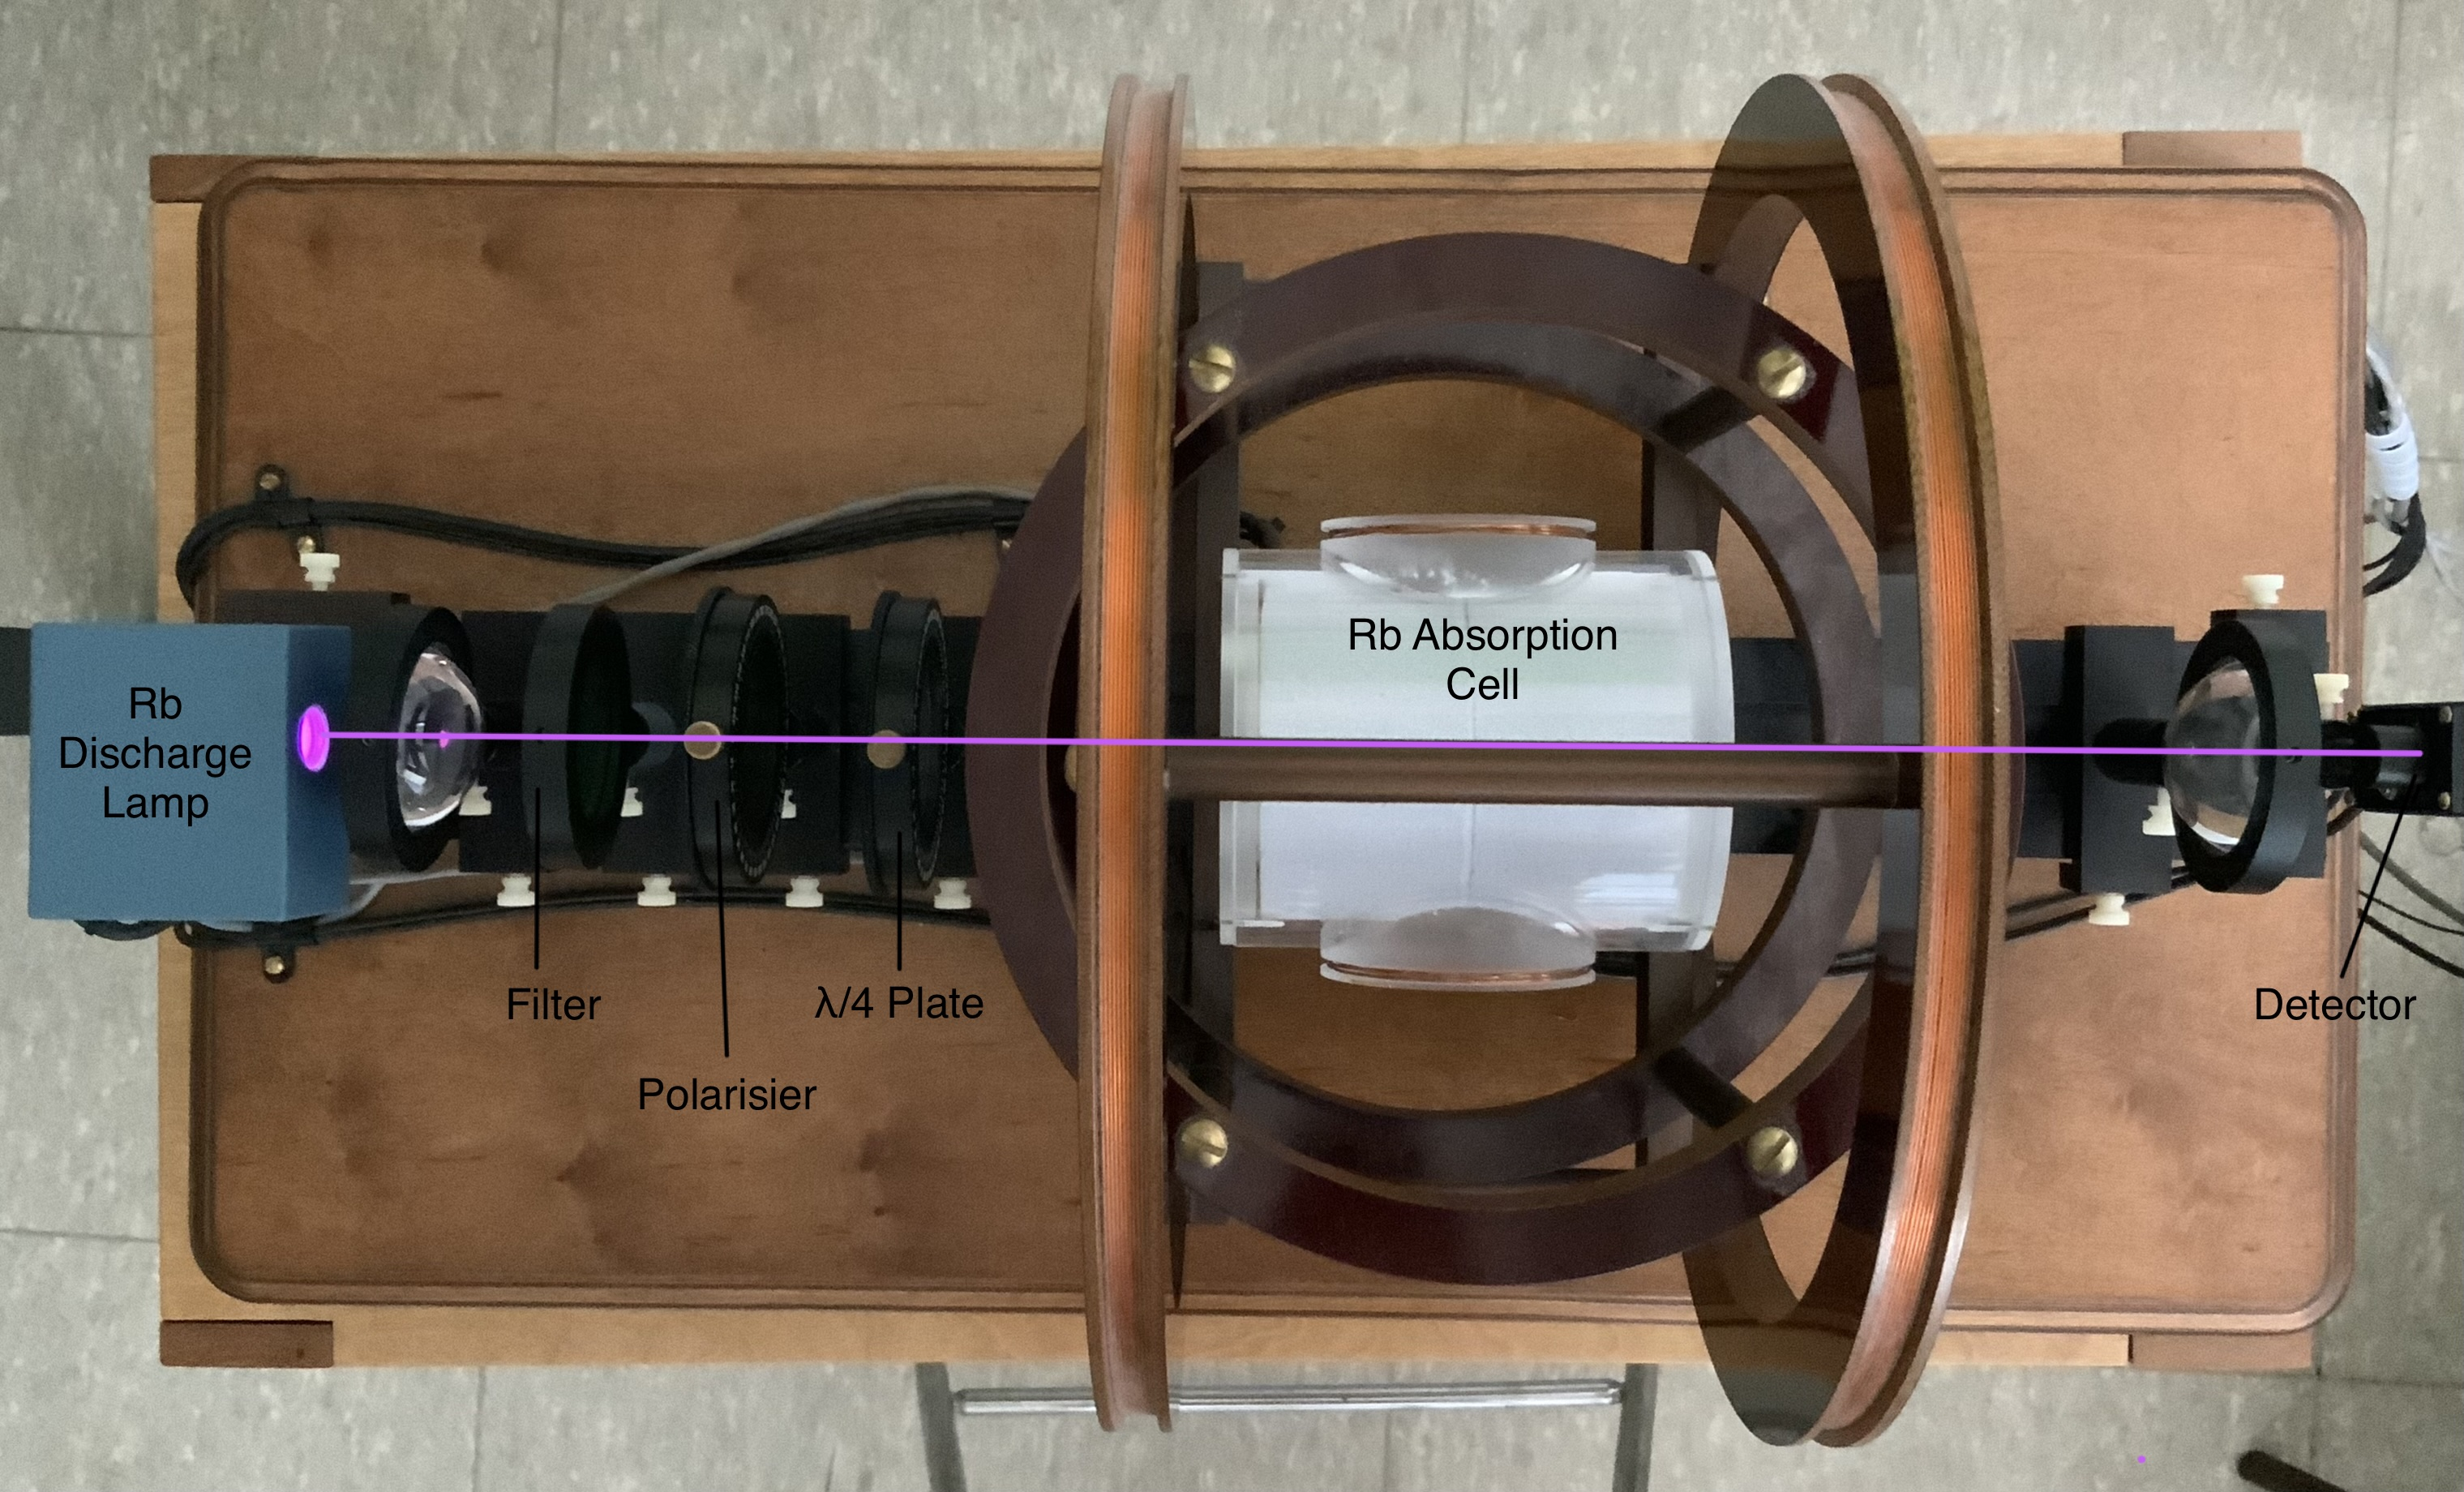
\includegraphics[width = .8\textwidth]{"content/pics/Aufbau.png"}
    \caption{Aufbau des Versuches \cite{v21}.}
    \label{fig:Aufbau}
\end{figure}

\subsection{Justage der Apparatur}
Vor dem Start der Messung wird die Rubidiumkammer vorgeheizt und die optischen Elemente so ausgerichtet, dass die Signalstärke des Photoelements
(Ausschlag des Galvanometers) maximiert wird. Anschließend wird der Versuchsaufbau mit einer Decke abgedeckt, um störende Einflüsse von äußerem Licht zu vermeiden.
Das Oszilloskop wird im XY-Modus betrieben, wobei die Modulation der RF Spule gegen den Photostrom des Photoelements aufgetragen wird. Ein breiter Peak bei 
$X = 0$ sollte nun sichtbar sein.
Mithilfe der Vertikalfeldspule kann die vertikale Komponente des Erdmagnetfeldes kompensiert werden. Dazu wird der Experimentiertisch in Nord-Süd Richtung 
ausgerichtet und der Strom der Vertikalfeldspule so eingestellt, dass die Breite des Nullpeaks minimal wird. Der eingestellte Strom kann zur Bestimmung der 
vertikalen Komponente des Erdmagnetfeldes verwendet werden.

\subsection{Messvorgang}
Zum ersten Teil der Messung werden die Werte der in \autoref{sec:Theorie} beschriebenen Resonanzfeldstärke $B_m$ in Abhängigkeit zur am Frequenzgenerator 
eingestellten Frequenz des RF Feldes bestimmt. Am Frequenzgenerator wird eine Sinusschwingung mit Frequenzen zwischen $\qty{100}{\kilo\hertz}$ und 
$\qty{1}{\mega\hertz}$ mit einer Schrittweite von $\qty{100}{\kilo\hertz}$ eingestellt. Mithilfe der Horizontalfeldspule und dem Startwert der Modulationsspule 
kann die Position der Transmissions-Einbrüche für beide Isotope bestimmt werden. Die jeweiligen Stromstärken der Spulen werden notiert.
Aus den erhaltenen Messwerten könenn die Landé-Faktoren $g_F$ für beide Isotope und die Kernspins $I$ bestimmt werden. \\

Für den zweiten Teil der Messung wird wieder eine Frequenz von $\qty{100}{\kilo\hertz}$ eingestellt und das Magnetfeld mithilfe des Startfeldes der Sweep Spule
auf eine Resonanzstelle eingestellt. Eine zusätzliche Rechteckspannung mit einer Periode von $\qty{5}{\hertz}$ wird auf die RF Spule angewendet, die für ein schnelles 
Ein- und Ausschalten des Feldes sorgt. Das Oszilloskop wird nun im Yt-Modus betrieben. Durch triggern auf die Kanten der RF-Modulation können der 
exponentielle Anstieg der Transmission und die Rabi-Oszillationen vermessen werden. Die Periodendauer der Rabi-Oszillationen wird in Abhängigkeit zur Amplitude des 
Funktionsgenerators vermessen.

